% ============================================================
%  MANUEL UTILISATEUR — manuel.tex
% ============================================================
\section{Manuel d'installation et d'utilisation}
\label{sec:manuel}

Cette section constitue le guide de référence destiné à toute personne souhaitant
installer, compiler et utiliser l'application Environnement. Les instructions
sont organisées de façon séquentielle~: prérequis, procédure de compilation,
lancement de l'application, puis guide d'utilisation de l'interface graphique.

% ------------------------------------------------------------
\subsection{Prérequis et environnement technique}
\label{subsec:prerequis}

Avant de procéder à l'exécution, il est nécessaire de vérifier que le Java
Development Kit (JDK)~8 ainsi que les bibliothèques listées dans le
tableau~\ref{tab:prerequis} sont présents sur la machine hôte. Un environnement
de développement intégré est également requis pour compiler le projet~; Eclipse
est recommandé car il a été utilisé lors du développement et garantit une
compatibilité optimale avec la configuration du projet.

\begin{table}[H]
  \centering
  \caption{Bibliothèques prérequises pour le bon fonctionnement de l'application}
  \label{tab:prerequis}
  \begin{tabular}{ll}
    \toprule
    \textbf{Bibliothèque} & \textbf{Rôle} \\
    \midrule
    jcommon       & Utilitaires communs JFreeChart \\
    hamcrest-core & Assertions pour les tests unitaires \\
    jfreechart    & Génération de graphiques 2D \\
    jfreesvg      & Export des graphiques au format SVG \\
    junit         & Framework de tests unitaires \\
    log4j         & Journalisation applicative \\
    swtgraphics2d & Pont entre SWT et Graphics2D \\
    \bottomrule
  \end{tabular}
\end{table}

L'application est compatible avec les systèmes d'exploitation Windows~10 ou
ultérieur, GNU/Linux (distributions Debian et dérivées) et macOS~12 ou ultérieur.
Une résolution d'écran d'au moins 1920\,$\times$\,1080~pixels est recommandée pour
un affichage optimal de l'interface graphique.

% ------------------------------------------------------------
\subsection{Récupération et compilation du projet}
\label{subsec:compilation}

La récupération du code source s'effectue via Git, puis la compilation est
réalisée depuis Eclipse.

\paragraph{Récupération du code source.}
La méthode recommandée est d'utiliser GitHub Desktop, qui simplifie la gestion du
dépôt. Après installation, le dépôt se clone via
\textit{File > Clone repository} en renseignant l'URL du projet~:

\begin{lstlisting}[style=java, language=bash, label=lst:clone,
    caption={Clonage du dépôt via GitHub Desktop}]
File > Clone repository > URL > coller l'URL du depot > Clone
\end{lstlisting}

Pour les utilisateurs ne souhaitant pas installer GitHub Desktop, il est possible
de télécharger le projet directement depuis l'interface web de GitHub~:

\begin{lstlisting}[style=java, language=bash, label=lst:zip,
    caption={Téléchargement du projet via l'interface web}]
Code > Download ZIP > extraire l'archive sur la machine locale
\end{lstlisting}

\paragraph{Compilation avec Eclipse.}
Une fois le projet récupéré, il convient de l'importer dans Eclipse en
suivant le chemin~:

\begin{lstlisting}[style=java, language=bash, label=lst:import,
    caption={Import du projet dans Eclipse}]
File > Import > Existing Projects into Workspace
  > selectionner le repertoire racine
\end{lstlisting}

Les bibliothèques listées dans le tableau~\ref{tab:prerequis} doivent ensuite être
ajoutées au build path~:

\begin{lstlisting}[style=java, language=bash, label=lst:buildpath,
    caption={Ajout des bibliothèques au build path}]
Project > Properties > Java Build Path > Add External JARs
\end{lstlisting}

La compilation s'effectue ensuite automatiquement à chaque sauvegarde si l'option
\textit{Build Automatically} est activée dans le menu \textit{Project}.

% ------------------------------------------------------------
\subsection{Lancement et utilisation de l'application}
\label{subsec:lancement}

Une fois le projet compilé conformément à la section~\ref{subsec:compilation},
l'application se lance depuis Eclipse en exécutant directement le fichier
\texttt{Environnement.java} via le menu~:

\begin{lstlisting}[style=java, language=bash, label=lst:run,
    caption={Lancement de l'application depuis Eclipse}]
Run > Run As > Java Application
\end{lstlisting}

Il est également possible de lancer l'application depuis un terminal si un fichier
\texttt{.jar} exécutable a été exporté au préalable via
\textit{File > Export > Runnable JAR file}~:

\begin{lstlisting}[style=java, language=bash, label=lst:runjar,
    caption={Lancement de l'application depuis un terminal}]
java -jar /chemin/vers/Environnement.jar
\end{lstlisting}

L'interface graphique s'ouvre automatiquement après quelques instants.

\paragraph{Étape 1 — Mode édition.}
Au lancement, la fenêtre d'édition s'affiche. Elle permet de configurer manuellement
la carte avant de démarrer la simulation. La figure~\ref{fig:manuel_edition}
présente l'aspect de cette fenêtre avec ses différentes zones de contrôle.

\begin{figure}[H]
  \centering
  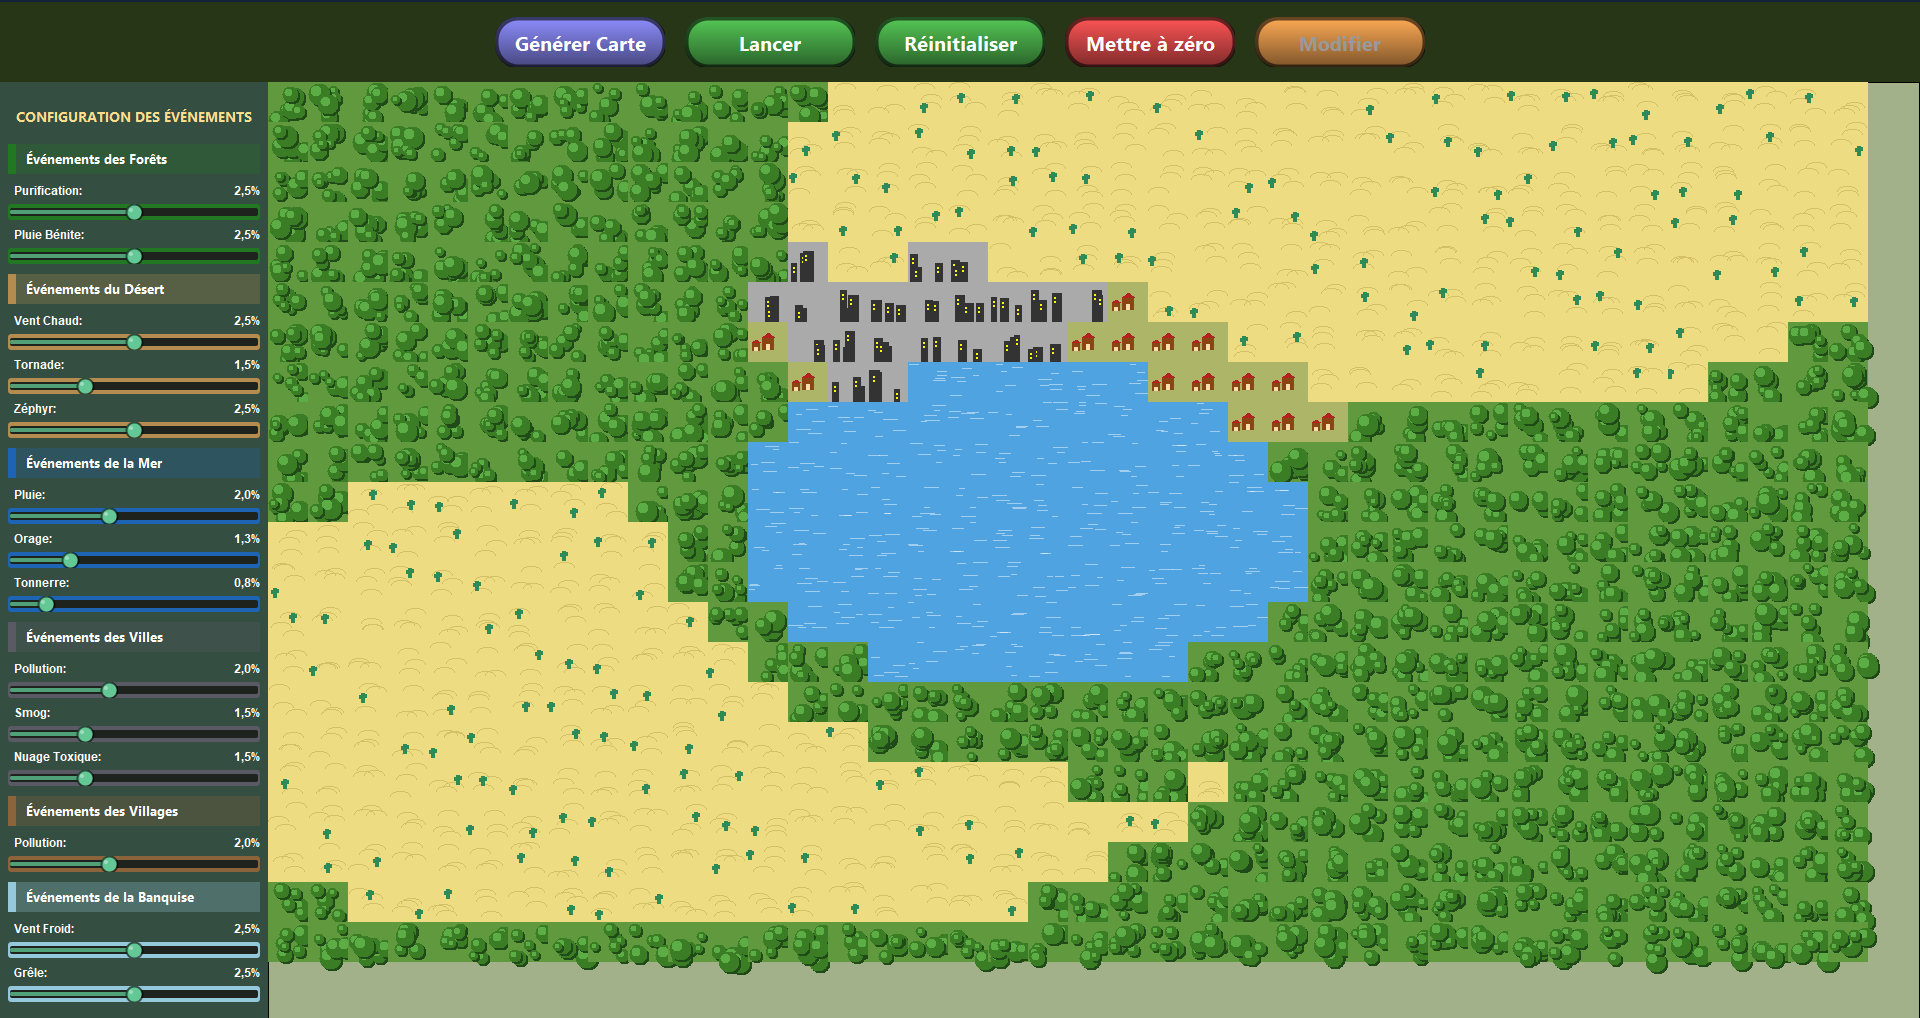
\includegraphics[width=0.85\textwidth]{images/image_edition}
  \caption{Fenêtre d'édition~: configuration de la carte et des probabilités
           d'événements}
  \label{fig:manuel_edition}
\end{figure}

Comme on peut le constater sur la figure~\ref{fig:manuel_edition}, les opérations
disponibles dans cette fenêtre sont les suivantes~:

\begin{itemize}
  \item modifier les probabilités qu'un événement survienne via le menu de gauche~;
  \item réinitialiser ou remettre à zéro les probabilités des événements avec les
    boutons \textit{Réinitialiser} ou \textit{Mettre à zéro}~;
  \item cliquer sur un biome pour ensuite changer sa nature avec le bouton
    \textit{Modifier}~;
  \item utiliser le bouton \textit{Génération aléatoire} pour remplir
    automatiquement la carte avec une distribution pseudo-aléatoire de biomes.
\end{itemize}

\paragraph{Étape 2 — Lancement de la simulation.}
Le bouton \textit{Lancer la simulation} ferme la fenêtre d'édition et ouvre la
fenêtre principale de simulation. La simulation débute automatiquement dès
l'ouverture de cette fenêtre.

\paragraph{Étape 3 — Contrôle de la simulation.}
Les contrôles disponibles dans le panneau inférieur (\texttt{PanelTemps})
permettent de piloter l'exécution. Le tableau~\ref{tab:controles} décrit chaque
bouton et son effet.

\begin{table}[H]
  \centering
  \caption{Contrôles de la simulation et leurs effets}
  \label{tab:controles}
  \begin{tabular}{ll}
    \toprule
    \textbf{Contrôle} & \textbf{Effet} \\
    \midrule
    \textit{Play}              & Démarre ou reprend la simulation après une pause \\
    \textit{Pause}             & Suspend l'exécution à la fin du round en cours \\
    \textit{Vitesse $\times 2$} & Double la cadence d'enchaînement des rounds \\
    \textit{Bilan de fin}      & Affiche un récapitulatif statistique de la simulation \\
    \textit{Statistiques}      & Ouvre la fenêtre d'analyse détaillée en temps réel \\
    \textit{Tutoriel}          & Ouvre la fenêtre d'aide et de présentation des règles \\
    \bottomrule
  \end{tabular}
\end{table}

\paragraph{Étape 4 — Lecture des statistiques.}
La figure~\ref{fig:manuel_simulation} illustre l'interface principale lors d'une
session en cours, avec ses trois zones fonctionnelles~: la grille centrale de
simulation, le panneau de statistiques et les contrôles de pilotage.

\begin{figure}[H]
  \centering
  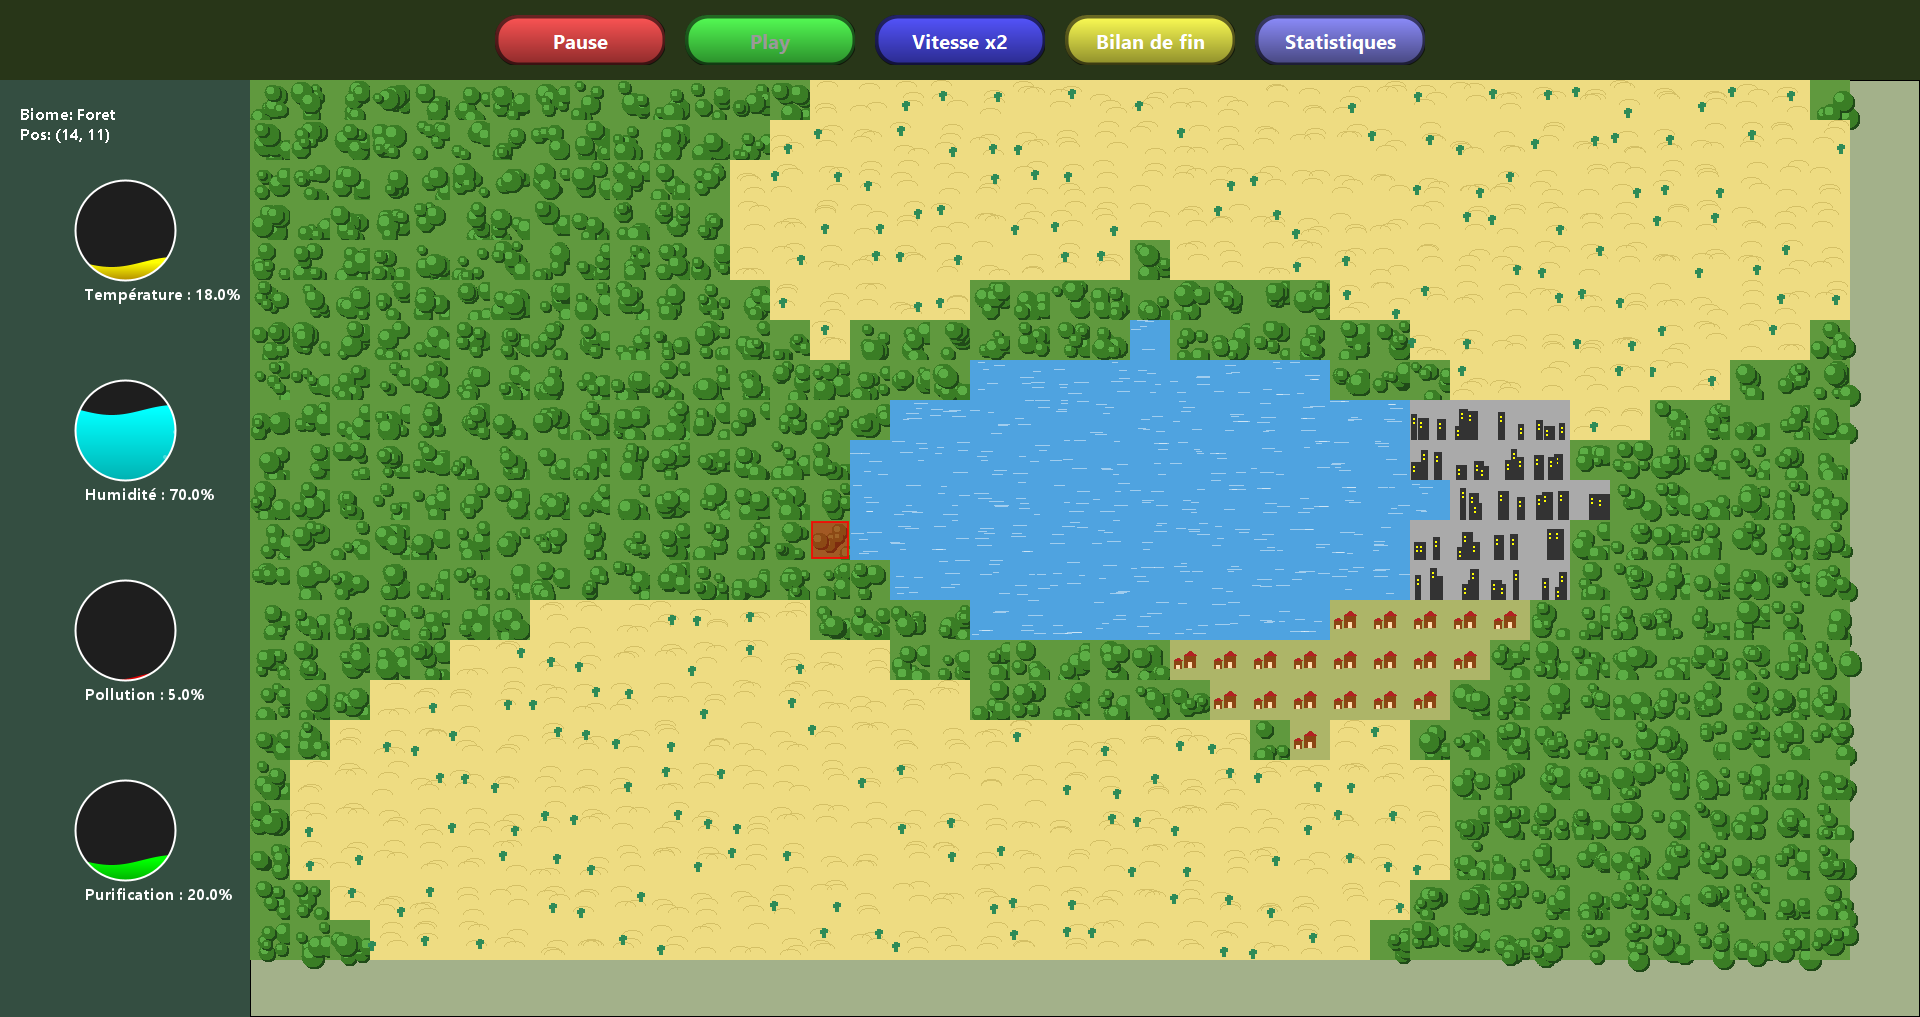
\includegraphics[width=0.9\textwidth]{images/image_simulation}
  \caption{Fenêtre principale de simulation~: grille, statistiques JFreeChart et
           contrôles}
  \label{fig:manuel_simulation}
\end{figure}

Tel qu'illustré dans la figure~\ref{fig:manuel_simulation}, le panneau latéral
droit affiche les statistiques en temps réel ainsi que les graphiques d'évolution
des propriétés générés par JFreeChart. En cliquant sur un biome de la grille
centrale, ses propriétés détaillées (température, humidité, pollution,
purification) s'affichent dans ce même panneau. La fenêtre \textit{Statistiques},
accessible depuis le tableau~\ref{tab:controles}, présente une analyse agrégée
de l'ensemble de la simulation sous forme graphique.

\paragraph{Consultation des journaux d'exécution.}
En cas d'anomalie ou à des fins d'analyse, les journaux de la session en cours sont
accessibles dans le fichier \texttt{src/logs/simulation.log}. Chaque entrée de
journal comporte un horodatage, un niveau de sévérité (\texttt{INFO} ou
\texttt{DEBUG}) et un message descriptif de l'action enregistrée.
